\clearpage
\chapter{Mastery Workbook 2}

% Chapter page
\section{Propositional Logic Workbook}

\horizontalline{0}{0}

\begin{center}
    \Large{\textbf{I have neither given nor received unauthorized assistance.}}
    \horizontalline{0}{0}
    \large{\textbf{Taylor James Larrechea}}
    \horizontalline{0}{0}
\end{center}

% Problem 1
\begin{problem}{Problem 1}
    \begin{statement}{Problem Statement}
        Before anything else, \textbf{annotate} examples 7 and 8 from page 30. You \textbf{MUST} use this \textbf{EXACT} format when showing logical equivalences (and proofs) to get credit for your work 
        in this course.
    \end{statement}

    Annotations can be seen on the next page.

    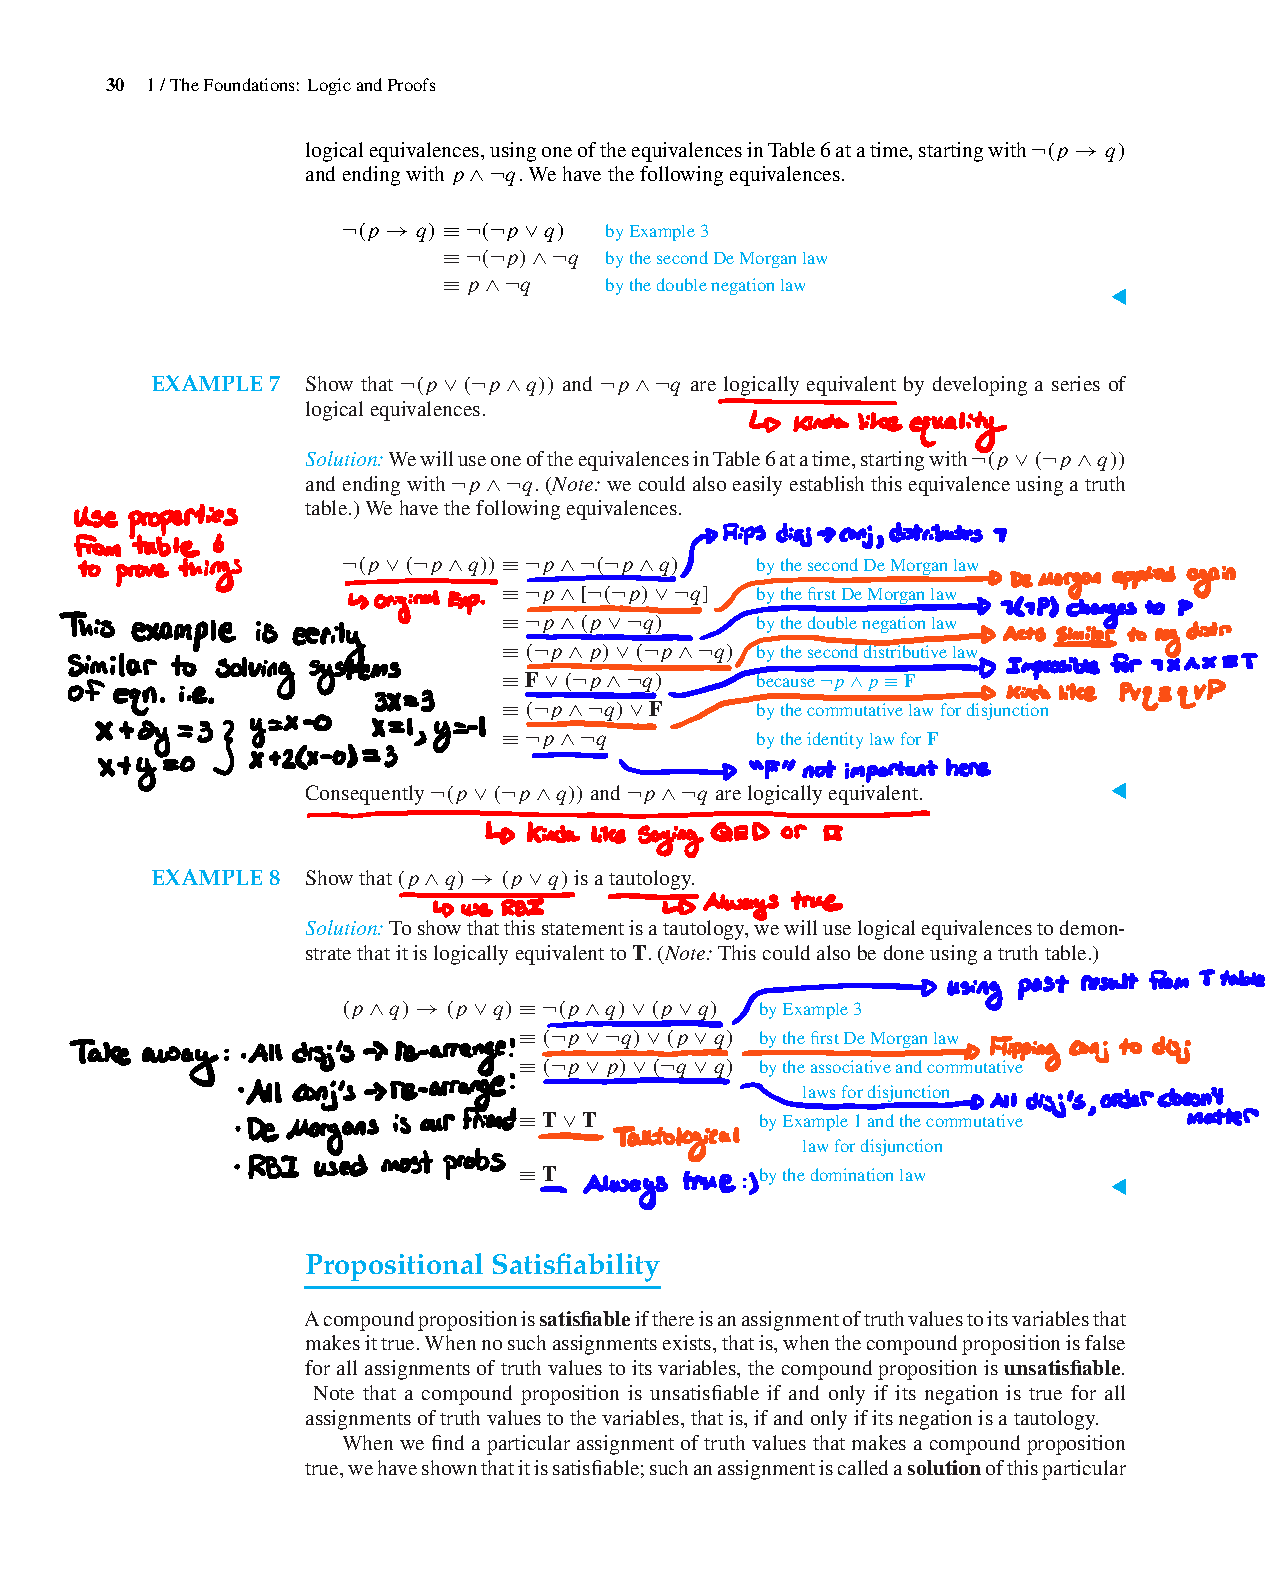
\includepdf[pages={-}, pagecommand={\thispagestyle{fancy}}, width=\paperwidth, offset=0 0]{./PDF/Annotations.pdf}
\end{problem}

% Problem 1 Summary
\begin{summary}{Problem 1 Summary}
    \begin{statement}{Procedure}
        \begin{itemize}
            \item Provide annotations for a proof format that is to be used in this class
        \end{itemize}
    \end{statement}
    \begin{statement}{Key Concepts}
        \begin{itemize}
            \item This problem involves the proper format that should be used for proofs in this class
            \item Always begin the proof with one side of the theorem, but \textbf{never} start a proof with what is to be proven
            \item Comments should be added to the right for each line of a proof
        \end{itemize}
    \end{statement}
    \begin{statement}{Variations}
        \begin{itemize}
            \item Because this problem involves annotating an example, a similar problem would be annotating a different problem
            \begin{itemize}
                \item In this case we would use the same procedure that was used in the original problem
            \end{itemize}
        \end{itemize}
    \end{statement}
\end{summary}

% Problem 2
\begin{problem}{Problem 2}
    \begin{statement}{Problem Statement}
        We will prove the first 5 logical equivalences in Chart 7 page 28.
        \begin{itemize}
            \item USE only RESULTS FROM \textbf{Chart 2 and Chart 6} to justify steps.
            \item When making logical chains of equivalences use the REQUIRED format.
            \item Prove these in this order and \textbf{you may use the results as you go.}
        \end{itemize}

        The logical equivalences that must be proven are:
        \begin{enumerate}[label=(\alph*)]
            \item This first one is what Chris calls RBI and it is essential because it converts a conditional into a disjunction. \textbf{Prove this with just a truth table.}
            \begin{equation*}
                p \rightarrow q \equiv \neg p \vee q
            \end{equation*}
            \item Carefully repeat the proof of the following using the method without a truth table from the video. Take note of what tricks Chris uses - as we will need these as we go. (Challenge - can 
            you prove it another way?)
            \begin{equation*}
                p \rightarrow q \equiv \neg q \rightarrow \neg p
            \end{equation*}
            \item Third one (hint: RBI works both ways).
            \begin{equation*}
                p \vee q \equiv \neg p \rightarrow q
            \end{equation*}
            \item Fourth one, (think about which rule `flips' conjunctions and disjunctions).
            \begin{equation*}
                p \wedge q \equiv \neg(p \rightarrow \neg q)
            \end{equation*}
            \item Finally, for the fifth one, see if you can do it on your own.
            \begin{equation*}
                \neg(p \rightarrow q) \equiv p \wedge \neg q
            \end{equation*}
        \end{enumerate}
    \end{statement}

    \begin{highlight}[Solution - Part (a)]
        We will first prove $p \rightarrow q \equiv \neg p \vee q$ with the use of a truth table.

        \begin{center}
            \begin{tabular}[h]{|c|c|c|c|c|}
                \hline $\mathbf{p}$ & $\mathbf{q}$ & $\mathbf{\neg p}$ & $\mathbf{p \rightarrow q}$ & $\mathbf{\neg p \vee q}$ \\ \hline
                T & T & F & T & T \\ \hline
                T & F & F & F & F \\ \hline
                F & T & T & T & T \\ \hline
                F & F & T & T & T \\ \hline
            \end{tabular}
        \end{center}
        Consequently, $p \rightarrow q$ is logically equivalent to $\neg p \vee q$.
    \end{highlight}

    \begin{highlight}[Solution - Part (b)]
        Starting with RBI, we can say

        \begin{align*}
            p \rightarrow q & \equiv \neg p \vee q & \text{(RBI)} \\
            & \equiv q \vee \neg p & \text{(Commutative Property)} \\
            & \equiv \neg q \vee \neg (\neg p) & \text{(Double Negation)} \\
            & \equiv \neg q \vee p & \text{(Double Negation Law)} \\
            & \equiv \neg q \rightarrow \neg p & \text{(RBI)}
        \end{align*}

        Consequently, $p \rightarrow q$ is logically equivalent to $\neg q \rightarrow \neg p$.
    \end{highlight}

    \begin{highlight}[Solution - Part (c)]
        Starting with RBI, we can say

        \begin{align*}
            \neg p \rightarrow q & \equiv \neg(\neg p) \vee q & \text{(RBI)} \\
            & \equiv p \vee q & \text{(Double Negation Law)}
        \end{align*}
        Consequently, $p \vee q$ and $\neg p \rightarrow q$ are logically equivalent.
    \end{highlight}

    \begin{highlight}[Solution - Part (d)]
        Starting with RBI, we can say

        \begin{align*}
            \neg(p \rightarrow \neg q) & \equiv \neg(\neg p \vee \neg q) & \text{(RBI)} \\
            & \equiv \neg(\neg p) \wedge \neg(\neg q) & \text{(De Morgans Law)} \\
            & \equiv p \wedge q & \text{(Double Negation Law)}
        \end{align*}
        Consequently, $p \wedge q$ and $\neg(p \rightarrow \neg q)$ are logically equivalent.
    \end{highlight}

    \begin{highlight}[Solution - Part (e)]
        Starting with RBI, we can say

        \begin{align*}
            \neg(p \rightarrow q) & \equiv \neg (\neg p \vee q) & \text{(RBI)} \\
            & \equiv \neg(\neg p) \wedge \neg q & \text{(De Morgans Law)} \\
            & \equiv p \wedge \neg q & \text{(Double Negation Law)}
        \end{align*}
        Consequently, $\neg(p \rightarrow q)$ and $p \wedge \neg q$ are logically equivalent.
    \end{highlight}

    \begin{highlight}[Insights]
        Most of these proofs started with RBI, where both De Morgan's Law and the Double Negation Law showed up frequently as well.
    \end{highlight}
\end{problem}

\begin{summary}{Problem 2 Summary}
    \begin{statement}{Procedure}
        \begin{enumerate}[label = (\alph*)]
            \item Part (a)
            \begin{itemize}
                \item Answer the truth values for each propositional statement and the final propositional statement
            \end{itemize}
            \item Part (b)
            \begin{itemize}
                \item Use RBI, Commutative Property, Double Negation Law to conclude the proof
            \end{itemize}
            \item Part (c)
            \begin{itemize}
                \item Use RBI and Double Negation to reach conclusion
            \end{itemize}
            \item Part (d)
            \begin{itemize}
                \item Use RBI, De Morgans Law, and Double Negation Law to reach conclusion
            \end{itemize}
            \item Part (e)
            \begin{itemize}
                \item Use RBI, De Morgans Law, and Double Negation Law to reach conclusion
            \end{itemize}
        \end{enumerate}
    \end{statement}
    \begin{statement}{Key Concepts}
        \begin{itemize}
            \item This problem uses several properties that can be applied to propositional statements and proves that two statements are equivalent to one another
            \item RBI (Rules By Inference) is $\alpha \rightarrow \beta \equiv \neg \alpha \vee \beta$ and is used to take a conditional statement and convert it to a disjunction
            \item De Morgans Law is $\neg (\alpha \vee \beta) \equiv \neg \alpha \wedge \neg \beta$ and $\neg (\alpha \wedge \beta) \equiv \neg \alpha \vee \neg \beta$ and is used in distributing a negation
            into a conjunction or disjunction
            \item Double Negation Law is $\neg (\neg \alpha) \equiv \alpha$ and is used to simplify a doubly negated proposition
        \end{itemize}
    \end{statement}
    \begin{statement}{Variations}
        \begin{itemize}
            \item We could be given a different propositional statement to prove
            \begin{itemize}
                \item In this case we would use the same properties with the new statement to prove the theorem that has been presented to us
            \end{itemize}
        \end{itemize}
    \end{statement}
\end{summary}

% Problem 3
\begin{problem}{Problem 3}
    \begin{statement}{Problem Statement}
        We can use Table 6 p.27 to prove new `rules'. Let’s prove a Logic version of the algebraic version FOIL. You will need to use a compound substitution with an equivalence from Table 6 twice. 
        (optional/recommended - create a truth table as well).
        \begin{equation*}
            (a \wedge b) \vee (c \wedge d) \equiv (a \vee c) \wedge (b \vee c) \wedge (a \vee d) \wedge (b \vee d)
        \end{equation*}
    \end{statement}

    \begin{highlight}[Solution]
        Starting with $(a \wedge b) \vee (c \wedge d)$, we can show

        \begin{align*}
            (a \wedge b) \vee (c \wedge d) & \equiv ((a \wedge b) \vee c) \wedge ((a \wedge b) \vee d) & \text{(Distributive Laws)} \\
            & \equiv (c \vee (a \wedge b)) \wedge (d \wedge (a \wedge b)) & \text{(Commutative Laws)} \\
            & \equiv ((c \vee a) \wedge (c \vee b)) \wedge ((d \vee a) \wedge (d \vee b)) & \text{(Distributive Laws)} \\
            & \equiv (c \vee a) \wedge (c \vee b) \wedge (d \vee a) \wedge (d \vee b) & \text{(Associative Laws)} \\
            & \equiv (a \vee c) \wedge (b \vee c) \wedge (a \vee d) \wedge (b \vee d) & \text{(Commutative Laws)}
        \end{align*}
        Consequently, $(a \wedge b) \vee (c \wedge d)$ and $(a \vee c) \wedge (b \vee c) \wedge (a \vee d) \wedge (b \vee d)$ are logically equivalent.

        $(a \wedge b)$ was treated as a single variable for the first line of this proof. Instead of complicating the above lines with another variable such as $\alpha$, I chose to wrap it with parenthesis
        to make the math clearer to me. After the second instance of the distributive law, I wrapped the disjunctions with parenthesis as well to make them resemble a single proposition instead of using a
        compound substitution.
    \end{highlight}
\end{problem}

% Problem 3 - Summary
\begin{summary}{Problem 3 Summary}
    \begin{statement}{Procedure}
        \begin{itemize}
            \item Use the Distributive law on the compound statement that is in the premise
            \item Use the Commutative and Associative Laws along with the Distributive law to reach the conclusion
        \end{itemize}
    \end{statement}
    \begin{statement}{Key Concepts}
        \begin{itemize}
            \item The Distributive law is $\alpha \vee (\beta \vee \gamma) \equiv (\alpha \vee \beta) \vee (\alpha \vee \gamma)$ and is used to distribute propositions in a statement
            \item The Commutative law is $\alpha \vee \beta \equiv \beta \vee \alpha$ and is used to rearrange propositions in a propositional statement
            \item The Associative law is used to remove parenthesis in a propositional statement to clean up the presentation of a statement
        \end{itemize}
    \end{statement}
    \begin{statement}{Variations}
        \begin{itemize}
            \item We could be asked to prove a different theorem with the same properties
            \begin{itemize}
                \item In this case we would use the same properties as before and use them to reach the final conclusion
            \end{itemize}
        \end{itemize}
    \end{statement}
\end{summary}

% Problem 4
\begin{problem}{Problem 4}
    \begin{statement}{Problem Statement}
        Rosen, page 53.  Do \#8 as warm-up on your own. Do \#9 below. Add notes and insight for full credit. \vspace*{1em}

        \textbf{9.)} Let $P(x)$ be the statement `$x$ can speak Russian' and let $Q(x)$ be the statement `$x$ knows the computer language C++.' Express each of these sentences in terms of $P(x)$, $Q(x)$, 
        quantifiers, and logical connectives. The domain for quantifiers consists of all students at your school.

        \begin{enumerate}[label=(\alph*)]
            \item There is a student at your school who can speak Russian and who knows C++.
            \item There is a student at your school who can speak Russian but who doesn't know C++.
            \item Every student at your school either can speak Russian or knows C++.
            \item No student at your school can speak Russian or knows C++.
        \end{enumerate}
    \end{statement}

    \begin{highlight}[Solution - Part (a)]
        `There is a student at your school who can speak Russian and who knows C++'.
        \setcounter{equation}{0}
        \begin{equation}
            \exists x (P(x) \wedge Q(x))
        \end{equation}
        Here we use $\exists$ to denote that over the entire domain of students, we are only concerned that there is at least one student who meets this criteria. We use $x$ to symbolize the domain of all
        students at the school and we use the conjunction `$\wedge$' to imply that the student knows Russian and C++. If the student knows Russian, $P(x)$ is true and if they know C++ as well, $Q(x)$ is true.
        The aforementioned statement will only be true if both $P(x)$ and $Q(x)$ applies to the current student.
    \end{highlight}

    \begin{highlight}[Solution - Part (b)]
        `There is a student at your school who can speak Russian but who doesn't know C++.'

        \begin{equation}
            \exists x (P(x) \wedge \neg Q(x))
        \end{equation}
        Similar to part (a), we once again use the existential quantifier to denote that we are only concerned if one or more students meet this criteria. Here, the only difference from part (a) is that we want 
        to implicate that this supposed student knows Russian but not C++. If $Q(x)$ applies to the student, then the aforementioned statement will be false, just as if $P(x)$ does not apply to the student. The 
        negation operator handles the scenario for when the student knows C++, the statement will also evaluate to false if the student does not know Russian.
    \end{highlight}

    \begin{highlight}[Solution - Part (c)]
        `Every student at your school either can speak Russian or knows C++.'

        \begin{equation}
            \forall x (P(x) \vee Q(x))
        \end{equation}
        In this example, we use $\forall$ to implicate that for the following statement to be true it must apply to all of the students at the school. After the universal quantifier, we include the domain of
        students to imply that for the disjunction $P(x) \vee Q(x)$ to be true, every student in the domain must either know Russian or C++. The statement will only evaluate to false for if there is a student
        that doesn't know Russian or C++.
    \end{highlight}

    \begin{highlight}[Solution - Part (d)]
        `No student at your school can speak Russian or knows C++.'

        \begin{equation}
            \forall x \neg(P(x) \vee Q(x))
        \end{equation}
        Finally, for this example we once again use the universal quantifier with the entire domain of students. We apply the negation operator `$\neg$' to imply that no student at the school can speak Russian
        or knows C++. If the inside expression $(P(x) \vee Q(x))$ evaluates to true, then this implies that there is a student that either knows Russian or C++. This in turn would cause the statement to evaluate
        to false because we are constituting that there is not a single student that this applies to.
    \end{highlight}
\end{problem}

\begin{summary}{Problem 4 - Summary}
    \begin{statement}{Procedure}
        \begin{enumerate}[label = (\alph*)]
            \item Part (a)
            \begin{itemize}
                \item Use the existential quantifier $\exists$ when dealing with a statement that has the phrase `There' or something similar in it
                \item Use a conjunction $\wedge$ when dealing with a statement that has the phrase `and' in it
            \end{itemize}
            \item Part (b)
            \begin{itemize}
                \item Use the existential quantifier $\exists$ when dealing with a statement that has the phrase `There' or something similar in it
                \item Use a conjunction $\wedge$ when dealing with a statement that has the phrase `but' in it
                \item Use a negation $\neg$ when dealing with a statement that has the phrase `doesn't' or something similar in it
            \end{itemize}
            \item Part (c)
            \begin{itemize}
                \item Use the universal quantifier $\forall$ when dealing with a statement that has the phrase `Every' or something similar in it
                \item Use a disjunction $\vee$ when dealing with a statement that has the phrase `or' in it
            \end{itemize}
            \item Part (d)
            \begin{itemize}
                \item Use the universal quantifier $\forall$ when dealing with a statement that has the phrase `no' or something similar in it
                \item Use a disjunction $\vee$ when dealing with a statement that has the phrase `or' in it
                \item Place the negation outside the propositions when the negation applies to the entire propositional statement
            \end{itemize}
        \end{enumerate}
    \end{statement}
    \begin{statement}{Key Concepts}
        \begin{itemize}
            \item Use the existential quantifier $\exists$ when dealing with a statement that is looking for a condition where there is at least one example of this being true
            \item Use the universal quantifier $\forall$ when dealing with a statement that is looking for a condition where it applies to everything in a statement
            \item Negations are placed based upon how they are supposed to negate a propositional statement or proposition alone
        \end{itemize}
    \end{statement}
    \begin{statement}{Variations}
        \begin{itemize}
            \item We could be given similar statements and asked to translate them into predicates and quantifiers
            \begin{itemize}
                \item In this case we would use the same procedure in determining how the and where to place the quantifiers and predicates with the correct logical connectives
            \end{itemize}
        \end{itemize}
    \end{statement}
\end{summary}

% Problem 5
\begin{problem}{Problem 5}
    \begin{statement}{Problem Statement}
        \#33 section 1.5, page 67 (add insights and comments for full credit). \vspace*{1em}

        \noindent \textbf{33.)} Rewrite each of these statements so that negations appear only within predicates (that is, so that no negation is outside a quantifier or an expression involving logical 
        connectives).

        \begin{enumerate}[label=(\alph*)]
            \item $\neg \forall x \forall y P(x,y)$
            \item $\neg \forall y \exists x P(x,y)$
            \item $\neg \forall y \forall x (P(x,y) \vee Q(x,y))$
            \item $\neg(\exists x \exists y \neg P(x,y) \wedge \forall x \forall y Q(x,y))$
            \item $\neg \forall x (\exists y \forall z P(x,y,z) \wedge \exists z \forall y P(x,y,z))$
        \end{enumerate}
    \end{statement}

    \begin{highlight}[Solution - Part (a)]
        Original expression: $\neg \forall x \forall y P(x,y)$.

        \setcounter{equation}{0}
        \begin{equation}
            \exists x \exists y \neg P(x,y) 
        \end{equation}
        These two expressions are logically equivalent because the original is making the claim that it is not the case that for all elements in the domain the predicate is true. This is the same as saying that in 
        the domain there is at least one case where the predicate is false.
    \end{highlight}

    \begin{highlight}[Solution - Part (b)]
        Original expression: $\neg \forall y \exists x P(x,y)$.

        \begin{equation}
            \exists x \forall y \neg (P(x,y))
        \end{equation}
        These two expressions are logically equivalent because the original is making the claim that it is not the case that for all elements in the domain $x$ and $y$ such that the predicate is true. This is the same 
        as saying that there is at least one element in the domain of $x$ for all elements in $y$ such that the predicate is false.
    \end{highlight}

    \begin{highlight}[Solution - Part (c)]
        Original expression: $\neg \forall y \forall x (P(x,y) \vee Q(x,y))$.

        \begin{equation}
            \exists y \exists x (\neg P(x,y) \wedge \neg Q(x,y))
        \end{equation}
        The original expression is conveying that it can't be the case that all elements in $x$ and $y$ satisfy the condition where either $P(x,y)$ or $Q(x,y)$ is true. The modified expression states that there is at least
        an element in $x$ and $y$ where both $P(x,y)$ and $Q(x,y)$ are false.
    \end{highlight}

    \begin{highlight}[Solution - Part (d)]
        Original expression: $\neg(\exists x \exists y \neg P(x,y) \wedge \forall x \forall y Q(x,y))$.

        \begin{equation}
            (\forall x \forall y P(x,y)) \vee (\exists x \exists y \neg Q(x,y))
        \end{equation}
        The simplest way I can attempt to explain this is that this is an example of how De Morgans Law applies to expressions with universal and existential quantifiers. Here, our conjunction flips to a disjunction and the 
        succeeding predicate $Q(x,y)$ is negated.
    \end{highlight}

    \begin{highlight}[Solution - Part (e)]
        Original expression: $\neg \forall x (\exists y \forall z P(x,y,z) \wedge \exists z \forall y P(x,y,z))$.

        \begin{equation}
            \exists x (\forall y \exists z \neg P(x,y,z) \vee \forall z \exists y \neg P(x,y,z))
        \end{equation}
        This is once again another example of De Morgans Law with predicates and quantifiers. I have noticed a pattern here, when a negation operator is carried through an expression, it will flip a existential quantifier to a 
        universal and vice versa. Here our conjunction flips to a disjunction and our predicates are negated via the De Morgans Law.
    \end{highlight}
\end{problem}

% Problem 5 Summary
\begin{summary}{Problem 5 Summary}
    \begin{statement}{Procedure}
        \begin{enumerate}[label = (\alph*)]
            \item Part (a)
            \begin{itemize}
                \item Flip the universal quantifiers to existential quantifiers when the negation appears in front of them
            \end{itemize}
            \item Part (b)
            \begin{itemize}
                \item Flip the universal quantifiers to existential quantifiers when the negation appears in front of them
                \item Flip the existential quantifiers to universal quantifiers when the negation appears in front of them
            \end{itemize}
            \item Part (c)
            \begin{itemize}
                \item Flip the universal quantifiers to existential quantifiers when the negation appears in front of them
                \item Apply De Morgans Law to the propositional statement with the predicates
            \end{itemize}
            \item Part (d)
            \begin{itemize}
                \item Flip the universal quantifiers to existential quantifiers when the negation appears in front of them
                \item Flip the existential quantifiers to universal quantifiers when the negation appears in front of them
                \item Apply De Morgans Law to the propositional statement with the predicates
                \item Always place the negation of a predicate after the quantifiers in a propositional statement
            \end{itemize}
            \item Part (e)
            \begin{itemize}
                \item Flip the universal quantifiers to existential quantifiers when the negation appears in front of them
                \item Flip the existential quantifiers to universal quantifiers when the negation appears in front of them
                \item Apply De Morgans Law to the propositional statement with the predicates
                \item Always place the negation of a predicate after the quantifiers in a propositional statement
            \end{itemize}
        \end{enumerate}
    \end{statement}
    \begin{statement}{Key Concepts}
        \begin{itemize}
            \item Negations flip universal quantifiers to existential quantifiers and vice versa
            \item De Morgans Law works with propositional statements involving predicates
            \item Always place the negation of a predicate after the quantifiers in a propositional statement
        \end{itemize}
    \end{statement}
    \begin{statement}{Variations}
        \begin{itemize}
            \item We could be given different statements with negations and asked how to apply them to the new statement
            \begin{itemize}
                \item We would use the same rules and procedures in determining what a negation does to quantifiers and propositional statements
            \end{itemize}
        \end{itemize}
    \end{statement}
\end{summary}

% Problem 6
\begin{problem}{Problem 6}
    \begin{statement}{Problem Statement}
        Now let’s go back to section 1.1. Read the examples on page 11 and 12 to see an important computer science application. Do each of \#43 and check your answers in the back of the book. Add notes and 
        insights. \vspace*{1em}

        \noindent \textbf{43.)} Find the bitwise \textit{OR}, bitwise \textit{AND}, and bitwise \textit{XOR} of each of these pairs of bit strings.

        \begin{enumerate}[label=(\alph*)]
            \item 101 1110, 010 0001
            \item 1111 0000, 1010 1010
            \item 00 0111 0001, 10 0100 1000
            \item 11 1111 1111, 00 0000 0000
        \end{enumerate}
    \end{statement}

    \begin{highlight}[Solution - Part (a)]
        Original: 101 1110, 010 0001.

        \setcounter{equation}{0}
        \begin{equation}
            \text{OR: 111 111} \hspace{10pt} \text{AND: 000 0000} \hspace{10pt} \text{XOR: 111 1111}
        \end{equation}
    \end{highlight}

    \begin{highlight}[Solution - Part (b)]
        Original: 1111 0000, 1010 1010

        \begin{equation}
            \text{OR: 1111 1010} \hspace{10pt} \text{AND: 1010 0000} \hspace{10pt} \text{XOR: 0101 1010}
        \end{equation}
    \end{highlight}

    \begin{highlight}[Solution - Part (c)]
        Original: 00 0111 0001, 10 0100 1000

        \begin{equation}
            \text{OR: 10 0111 1001} \hspace{10pt} \text{AND: 00 0100 0000} \hspace{10pt} \text{XOR: 10 0011 1001}
        \end{equation}
    \end{highlight}

    \begin{highlight}[Solution - Part (d)]
        Original: 11 1111 1111, 00 0000 0000

        \begin{equation}
            \text{OR: 11 1111 1111} \hspace{10pt} \text{AND: 00 0000 0000} \hspace{10pt} \text{XOR: 11 1111 1111}
        \end{equation}
    \end{highlight}

    \begin{highlight}[Solution Insights]
        This problem seemed to be really easy for me. In the bitwise OR, the corresponding truth value will be 1 if either bits are a 1 and will be 0 if both bits are 0. For the AND, both bits of the bit strings that are being 
        compared must be 1 for it to be 1 and otherwise it will be 0. For the XOR, when comparing the strings, the comparison will only be 1 if one bit from one string is a 1 and the other is a 0. Otherwise, if both are 1's or 
        both are 0's then XOR will evaluate to 0.
    \end{highlight}
\end{problem}

% Problem 6 Summary
\begin{summary}{Problem 6 Summary}
    \begin{statement}{Procedure}
        \begin{itemize}
            \item If either bit is a 1 in bitwise OR, then place a 1 for that value, 0 otherwise
            \item If both bits are 1's in bitwise AND, then place a 1 for that value, 0 otherwise
            \item If one bit is a 1 and the other is a 0 in bitwise XOR, then place a 1 for that value, 0 otherwise
        \end{itemize}
    \end{statement}
    \begin{statement}{Key Concepts}
        \begin{itemize}
            \item Bitwise OR evaluates to 1 if either bit is a 1
            \item Bitwise AND evaluates to 1 if both bits are a 1
            \item Bitwise XOR evaluates to 1 if and only if 1 bit is a 1 and the other is a 0
        \end{itemize}
    \end{statement}
    \begin{statement}{Variations}
        \begin{itemize}
            \item We could be given different strings of bits to evaluate the truth value of each operation
            \begin{itemize}
                \item We would then use the same rules for each operation to find the truth value of each bit
            \end{itemize}
        \end{itemize}
    \end{statement}
\end{summary}